\begin{figure}[t]
    \centering
    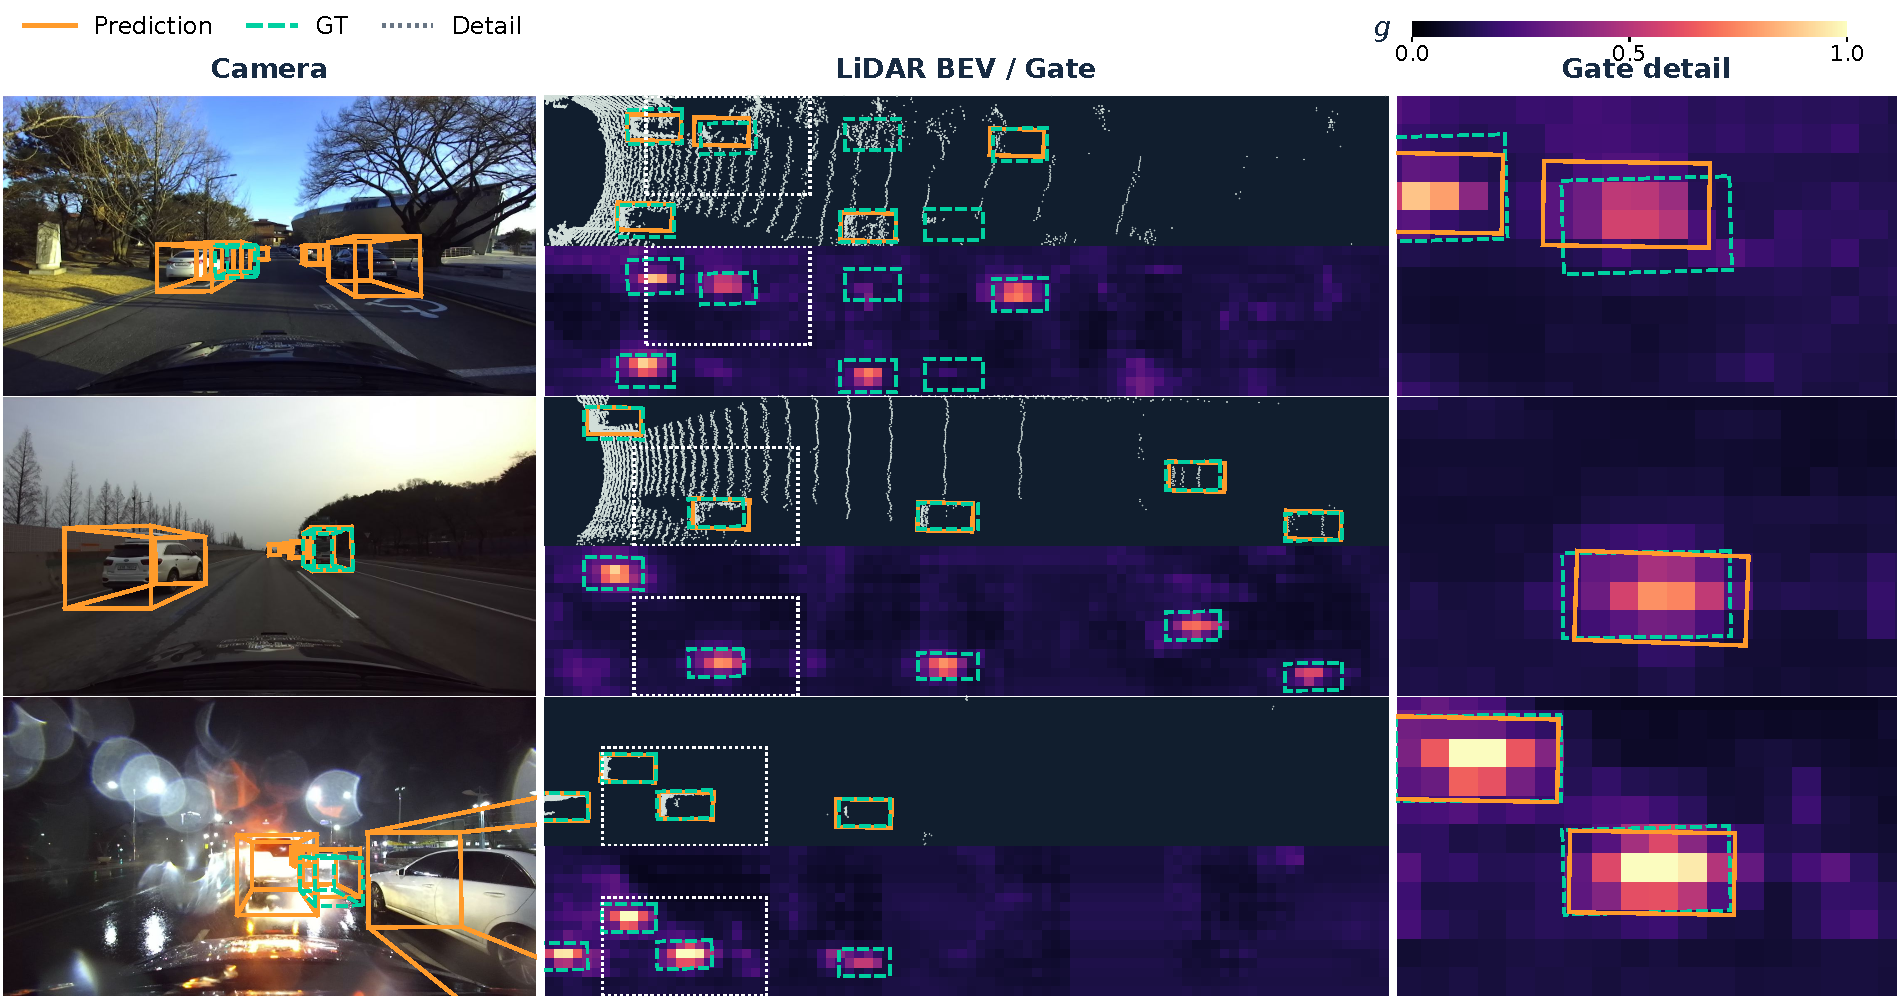
\includegraphics[width=\linewidth]{assets/figure4.pdf}
    \caption{Spatial gating and detection in matched scenes. Each row shows the camera image with ObjDec predictions (left), the full LiDAR BEV and predicted foreground gate (middle, top and bottom), and a magnified gate region (right). Orange solid and green dashed boxes denote predictions with scores above 0.3 and GT references, respectively. Camera panels show the selected target's GT; the BEV and gate panels retain all GT references within their displayed regions. White dotted rectangles mark detail windows. Full BEV views cover $x\in[0,72]$ m and $y\in[-6.4,6.4]$ m; right-hand windows span $14\times8.4$ m, with forward $x$ horizontal and lateral $y$ vertical. All gates use the native 0.8 m grid and a common $[0,1]$ scale without smoothing. Foreground/background gate means are 0.213/0.128, 0.259/0.115, and 0.288/0.118 from top to bottom. Gates are predicted directly from features; GT overlays and region statistics are added after prediction. Gate values modulate fusion and are distinct from detection confidence.}
    \label{fig:4}
\end{figure}
